\documentclass{beamer}

\title{TREAT}
\subtitle{Timed Regular Expression to Automaton Transformation}
\author{Group 30}
\institute{Aalborg Universitet}
\date{2024}

\title{TREAT}
\subtitle{Timed Regular Expression to Automaton Transformation}
\author{Group 30}
\institute{Aalborg Universitet}
\date{2024}

\usepackage{tikz-uml}
\usepackage[T1]{fontenc}
\usepackage{listings}
\usetikzlibrary {automata,positioning}
\usepackage{xcolor}

\usetheme{Frankfurt}
\useinnertheme{rectangles}
% \setbeamertemplate{footline}[frame number]
\addtobeamertemplate{navigation symbols}{}{%
    \usebeamerfont{footline}%
    \usebeamercolor[fg]{footline}%
    \hspace{1em}%
    \insertframenumber/\inserttotalframenumber
}

\begin{document}


\frame{\titlepage}

\begin{frame}{Agenda}
    \tableofcontents
\end{frame}

\section{Introduction} % each section gets own category on top bar, each frame within gets a subcategory
\begin{frame} {Process}

\end{frame}

\section{Implementation}
\begin{frame}{UPPAAL}
    \begin{columns}
        \begin{column}{0.4\textwidth}
            \begin{itemize}
                \item UML
                \item Structured using UPPAAL .dtd
            \end{itemize}
        \end{column}
        \begin{column}{0.6\textwidth}
            \scalebox{0.8}{
                \scalebox{0.5}{\begin{tikzpicture}
        \umlclass[anchor=north,width=31ex,x=0,y=0]{nta}{system : string}{}

        %classes
        \umlclass[anchor=north,width=31ex,x=0,y=-4.3]{template}{name : string\\ init : string}{}
        \umlclass[anchor=north,width=31ex,x=-6,y=-9]{declaration}{clocks : list<string>\\channels : list<char>}{}

        %relations
        \umlcompo[attr1=1|,attr2=1..*|,pos2=0.87]{nta}{template}
        \umlHVcompo[attr1=1|,attr2=1|,pos1=0.1,pos2=1.98]{nta}{declaration}
        \umlHVcompo[attr1=1|,pos1=0.1,pos2=1.98]{template}{declaration}

        %classes
        %\umlclass[x=-6,y=-6]{parameter}{}{}
        %\umlclass[x=-3,y=-6]{branchpoint}{}{}
        \umlclass[anchor=north,width=31ex,x=0,y=-9]{location}{id : string\\name : string}{}
        \umlclass[anchor=north,width=31ex,x=6,y=-9]{transition}{source : string\\target : string}{}
        %\umlclass[x=15,y=-6]{parameter}{}{}
        %relations
        \umlcompo[attr1=1|,attr2=0..*|,pos1=0.15,pos2=0.9]{template}{location}
        \umlHVcompo[attr1=1|,attr2=0..*|,pos1=0.1,pos2=1.95]{template}{transition}
        %\umlVHVcompo[attr2=0..1|,pos2=2.75]{template}{parameter}

        %classes
        \umlclass[anchor=north,width=31ex,x=0,y=-14]{label}{kind : string\\ content : string}{}
        %relations
        \umlcompo[arg1=1,arg2=0..*,pos1=0.15,pos2=0.9]{location}{label}
        \umlVHcompo[arg1=1,arg2=0..*,pos1=0.1,pos2=1.9]{transition}{label}

        %classes
        %\umlclass[x=-6,y=-9]{committed}{}{}
        %\umlclass[x=-9,y=-9]{urgent}{}{}
        %relationsde
        %\umlVHVcompo[attr2=0..1|,pos2=2.75]{location}{committed}
        %\umlVHVcompo[attr2=0..1|,pos2=2.75]{location}{urgent}
    \end{tikzpicture}}


            }
        \end{column}
    \end{columns}
    % \hspace{10em}

\end{frame}
\begin{frame}[fragile]{UPPAAL}
    \definecolor{bluekeywords}{rgb}{0,0,1}
    \definecolor{greencomments}{rgb}{0,0.5,0}
    \definecolor{redstrings}{rgb}{0.64,0.08,0.08}
    \definecolor{xmlcomments}{rgb}{0.5,0.5,0.5}
    \definecolor{types}{rgb}{0.17,0.57,0.68}

    \lstset{language=[Sharp]C,
        captionpos=b,
        %numbers=left, %Nummerierung
        %numberstyle=\tiny, % kleine Zeilennummern
        frame=lines, % Oberhalb und unterhalb des Listings ist eine Linie
        showspaces=false,
        showtabs=false,
        breaklines=true,
        showstringspaces=false,
        breakatwhitespace=true,
        commentstyle=\color{greencomments},
        morekeywords={partial, var, value, get, set},
        keywordstyle=\color{bluekeywords},
        stringstyle=\color{redstrings},
        basicstyle=\ttfamily\tiny,
    }
    \begin{lstlisting}
internal Nta()
{
    _templates = new List<Template>();
    Declaration = new Declaration(new List<string>(), new List<string>());
}    
    \end{lstlisting}
    \vspace{1em}
    \begin{lstlisting}
internal Template(...)
{
    Declaration = declaration;
    Declaration.AddClocks(clocks);
    Name = name;
    Init = init;
    _locations = locations.ToArray();
    _transitions = transitions.ToArray();
}  
    \end{lstlisting}
\end{frame}

\begin{frame}{Demonstration}

\end{frame}

\section{Discussion}
\begin{frame}{Future works}
    \begin{columns}
        \begin{column}{0.4\textwidth}
            \begin{itemize}
                \item Pruning
                \item <4>TA $\rightarrow$ TRE
            \end{itemize}
        \end{column}
        \begin{column}{0.6\textwidth}
            \visible<2-3> {
                \scalebox{0.8}{
                    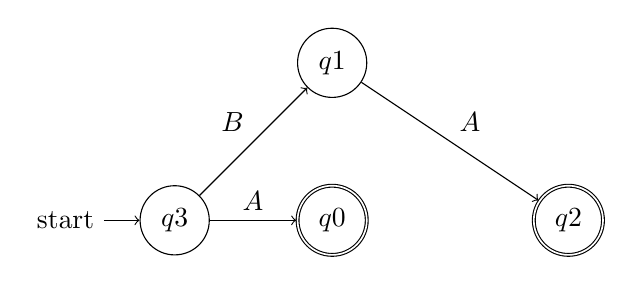
\begin{tikzpicture}[auto]
                        \node[state, accepting] at (2, 0)(q0){$q0$};
                        \node[state] at (2, 2)(q1){$q1$};
                        \node[state, accepting] at (5, 0)(q2){$q2$};
                        \node[state, initial] at (0, 0)(q3){$q3$};

                        \path[->]
                        (q1)edge node{$A$}(q2)
                        (q3)edge node{$A$}(q0)
                        (q3)edge node{$B$}(q1)
                        ;
                    \end{tikzpicture}
                }
            }

            \vspace{2em}
            \visible<3> {
                \scalebox{0.8}{
                    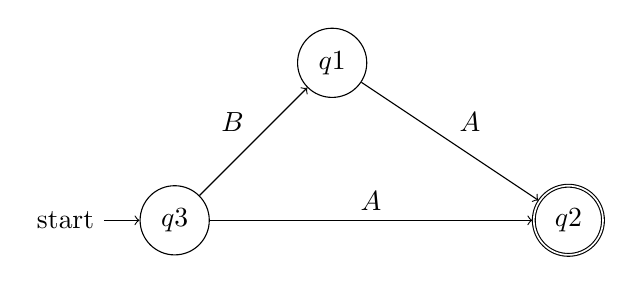
\begin{tikzpicture}[auto]
                        \node[state, accepting] at (5, 0)(q2){$q2$};
                        \node[state] at (2, 2)(q1){$q1$};
                        \node[state, initial] at (0, 0)(q3){$q3$};

                        \path[->]
                        (q1)edge node{$A$}(q2)
                        (q3)edge node{$A$}(q2)
                        (q3)edge node{$B$}(q1)
                        ;
                    \end{tikzpicture}
                }
            }
        \end{column}
    \end{columns}
\end{frame}
\begin{frame}{Enhancements}
    \begin{itemize}
        \item Bugfixes after hand-in
              \begin{itemize}
                  \item int32 indices
                  \item graph layout crashes
                  \item $\cdots$
              \end{itemize}
    \end{itemize}

\end{frame}
\begin{frame}{Learning Goals}
    \begin{itemize}
        \item is this relevant? genuine question
    \end{itemize}
\end{frame}
\section{Conclusion}
\begin{frame}{Conclusion}
    \begin{itemize}
        \item TREAT
        \item Readability
    \end{itemize}
\end{frame}

\end{document}